\documentclass[tikz]{standalone}
\usepackage{tikz}
\usetikzlibrary{shapes,decorations,arrows,calc,arrows.meta,fit,positioning}
\tikzset{
    -Latex,auto,node distance =1 cm and 1 cm,semithick,
    state/.style ={ellipse, draw, minimum width = 0.7 cm},
    point/.style = {circle, draw, inner sep=0.04cm,fill,node contents={}},
    bidirected/.style={Latex-Latex,dashed},
    el/.style = {inner sep=2pt, align=left, sloped}
}

\begin{document}
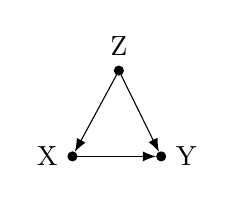
\begin{tikzpicture}[scale=1.0]
\node (X) [label = left:X, point];
\node (Y) [label = right:Y, point, right = of X];
\node (Z) [label = above:Z, xshift=-0.5cm, point, above right = of X];

\path (X) edge (Y);
\path (Z) edge (X);
\path (Z) edge (Y);

\end{tikzpicture}

\end{document}
